\chapter{Fall dynamics}\label{ChapAppendFallDynamics}

There are several models of the fall dynamics of ash particles that have
been implemented in Ash3d.  All calculate the fall velocity of a particle
according to the following equation \cite[p.182]{Bird60}:
\begin{equation}
v_s=\sqrt{\frac{4d\rho g}{3C_d\rho_a}}\label{EqFallVel}
\end{equation}
This formula requires a particle diameter and density ($d$ and $\rho$),
air density $\rho_a$, and the drag coefficient, $C_d$.
The various fall models differ in their
specification of $C_d$, but generally are functions of $\mathrm{Re}$
and are variations of the Stoke's Law
for spherical particle at low $\mathrm{Re}$.
\begin{equation}
C_d = \mathcal{F}(\mathrm{Re}) = \frac{24}{\mathrm{Re}}\label{EqCdStokes}
\end{equation}
The particle Reynold's number $\mathrm{Re}$, is given by 
\begin{equation}
\mathrm{Re}=\frac{v_s\rho_a d}{\eta_a}\label{EqReyn}
\end{equation}
where $\eta_a$ is the viscosity of air.  Given an arbitrary function
for $C_d$, the three equations \ref{EqFallVel} through \ref{EqReyn}
require an iteritive approach to solving for $v_s$.  Ash3d implements
this solver by initializing the fall velocity to $1 \, \mathrm{m/s}$,
solving for the corresponding $\mathrm{Re}$ via \ref{EqReyn}, then
calculating $C_d$ via the particular fall model, and then updating
$v_s$ via \ref {EqFallVel}.  This process repeats until $v_s$ changes
by less than 0.1\%.

Several atmospheric quantities are needed to calculate the fall velocity,
primarily the density and viscosity of air.
The density is calculated via the ideal gas law and the viscosity via
Sutherland's Law \cite[p.102, Eq.4.54]{Jacobson05}
\begin{equation}
\eta_a= 1.8325 \times 10^{-5} \left( \frac{416.16}{T+120}\right) 
\left( \frac{T}{296.16}\right)^{1.5}
\end{equation}

For conditions where $\rho_a$
is low and particle size is small, the mean free path of a molecule in the
atmosphere, $\lambda_a$, can be on the scale of the particle diamter.  For these
conditions an additional modification to the expression for $C_d$ can
be invoked by scaling $C_d$ by the the Cunninghan slip-correction factor
\begin{equation}
C_c = 1+\mathrm{Kn}\left[\alpha+\beta \exp{\left(-\frac{\gamma}{\mathrm{Kn}}\right)} \right]\label{EqCc}
\end{equation}
where the particle Knudsen number is given by $\mathrm{Kn}=2 \lambda_a / d$.
Ash3d uses values for the empirical coefficients $\alpha$, $\beta$, and
$\gamma$ given by \cite[p.407, Eq.9.34]{Seinfeld06}.
The air mean free path, $\lambda_a$, is given by \cite[p.399, Eq.9.6]{Seinfeld06}:
\begin{equation}
\lambda_a = \frac{2 \eta_a}{P\sqrt{8M_B/\pi R T}}\label{EqLambda}
\end{equation}

For spherical particles in the low $\mathrm{Re}$ region,
the Stokes fall model (\texttt{FV\_ID=5}) can be used, and $C_d$ is calculated
according to Eq. \ref{EqCdStokes}.  For non-spherical particles, Ash3d
has implemented the Wilson and Huang model (with optional modifications for
slip and following Pfeiffer et al) and the Ganser model.

The Wilson and Huang model uses $C_d$ according to
\begin{equation}
C_d = \frac{24}{\mathrm{Re}}F^{-0.828}+2 \sqrt{1.07-F}\label{EqDragWH}
\end{equation}
where $F$ is a shape parameter for an ellipsoidal particle
defined as the ratio of the average of the minor axes to the major axis of
the particle:  $(B+C)/2A$. 

If using the Cunningham slip-flow correction, for ellipsoidal particles,
Eq. \ref{EqCc} must be adjusted by scaling
$\mathrm{Kn}$ according to \cite[Table 1]{Dahneke73c}.

Equation \ref{EqDragWH} was empirically determined from fall data from volcanic
particles in the size range $30 \, \mathrm{\mu m} < d < 1500 \, \mathrm{\mu m}$
where $d$ is the
arithmetic mean of the ellipsoid diameters ($d=d_a=(A+B+C)/3$).  The slip-flow
correction only becomes significant for particles smaller than this range.
In this model, oblate and prolate ellipsoids can have the same shape parameter,
as for example the ellipsoids ($A=1.0$, $B=0.5$, $C=0.5$) and 
($A=1.0$, $B=0.9$, $C=0.1$), both of which have $F=0.5$.

The Ganser model is more sophisticated in that prolate and oblates ellipsoids
can be distinguished using a second shape parameter.  Ash3d uses a first
shape parameter of $F=(B+C)/2A$, and an optional second $G=C/B$ which describes
the ratio of the minor to intermediate axes of the ellipse.  If $G$ is not
provided, it is assumed to be $1$, meaning $B=C$ (prolate spheroids only).
The drag coefficient for the Ganser model is given by
%Figure \ref{FigFallVel} shows the fall velocity models as a function of particle
%size for prolate ellipsoidal particles ($F=0.4$) as well as for more equant
%particles ($F=0.8$) using atmospheric conditions at a height of $10 \,\mathrm{km}$.
%The Ganser model is also shown for comparison.  The Wilson and Huang model predicts
%slightly slower settling velocities than the Ganser model and the Stokes' model
%(by $53\%$ and $17\%$ for $F=0.4$ and $F=0.8$, respectively).  For $F=0.4$, the
%slip-flow corections are minor, however for $F=0.8$, it leads to increases in fall
%velocities by $2\%$, $21\%$, and $348\%$ for $d=10 \,\mathrm{\mu m}$, $1 \,\mathrm{\mu m}$
%and $0.1 \,\mathrm{\mu m}$ respectively.
%\cite{Rose09} calculated that ash in this size range can be a significant component
%($30\%$ to $>50\%$) of the total grain size distribution and noted that sedimentation
%rates are observed to be be much faster than that predicted by Stokes' Law.
\begin{equation}\label{EqFVGansCd}
C_d = \frac{24}{\mathrm{Re}K_1} \left( 1 + 0.1118 \left(\mathrm{Re} K_1 K_2 \right)^{0.6567}\right)
+ \frac{0.4305 K_2}{1+ \frac{3305}{\mathrm{Re} K_1 K_2}}
\end{equation}
where the Stokes and Newton shape factors ($K_1$ and $K_2$, respectively)
are functions of the sphericity, $\phi$, defined as
the ratio of the surface area of a sphere with equivalent particle volume to
the actual surface area of the particle.  
\begin{equation}\label{EqFVGansK1}
K_1 = \left( \frac{1}{3} +\frac{2}{3}\phi^{-1/2}  \right)^{-1}
\end{equation}
\begin{equation}\label{EqFVGansK2}
K_2 = 10^{1,8148 \left( -\log \phi \right)^{0.5743}}
\end{equation}

Both Eq.s \ref{EqDragWH} and \ref{EqFVGansCd} have a first term that is a
perturbation on the Stoke's flow drag (Eq. \ref{EqCdStokes}) which is the
dominant term for low $\mathrm{Re}$ flows 
The second additive term in these drag models becomes
dominant for high $\mathrm{Re}$ flows (Stoke's and Newton regimes,
respectively).  If we normalize the ellipsoid diamters to the major axes,
$A$, as $B=\beta A$ and $C=\gamma A$, then we can
express these in terms of $F$ and $G$ as
\begin{eqnarray}\label{EqShapeBetaGamma}
\beta &= \frac{2F}{1+G} \\
\gamma&= \frac{2FG}{1+G}
\end{eqnarray}
We can then calculate the diameter of
a sphere of equivalant volume as
\begin{equation}\label{EqDv}
d_v = \sqrt[3]{ABC} = A \sqrt[3]{\beta \gamma}
\end{equation}
Then using the approximate formula for the surface area of an ellipsoid
\begin{equation}\label{EqAreaEllipsoid}
S \sim 4 \pi \sqrt[p]{\frac{(ab)^p + (ac)^p + (bc)^p}{3}}
\end{equation}
where $a$, $b$, and $c$ are the major, intermediate, and minor radii, and 
$p \approx 1.6075$ \cite{WikiEllipse}.  This results in a sphericity of
\begin{equation}\label{EqSpericity}
\phi = \frac{A_{sphere}}{A_{particle}} =\left( \beta \gamma \right)^{\frac{2}{3}}
\left[ \frac{\beta^p + \gamma^p + \left( \beta \gamma \right)^p}{3} \right]^{-\frac{1}{p}}
\end{equation}
Particle diameter in the Ganser model is based on the equivalent volume sphere which
is the geometric average of the partical diameters given in Eq. \ref{EqDv}.

As mentioned, most of these fall models require an iterative approach to solving
for $v_s$.  The exception is the Wilson and Huang model without the slip-correction,
for which there is an explicit solution to a quadratic expression.  Since the
other fall models can be computationally expensive, the atmospheric parameters
($\rho_a$, $\eta_a$, $\lambda_a$) are only calculated on the nodes of the
meteorological grid (not the computational grid).  Fall velocities for each
bin are calculated on these meteorological nodes,
then interpolated to the computational grid.
For this approximation to be valid, the density and viscosity of air must not
be strongly non-linear between the meteorological grid nodes.

\begin{figure}[htbp]
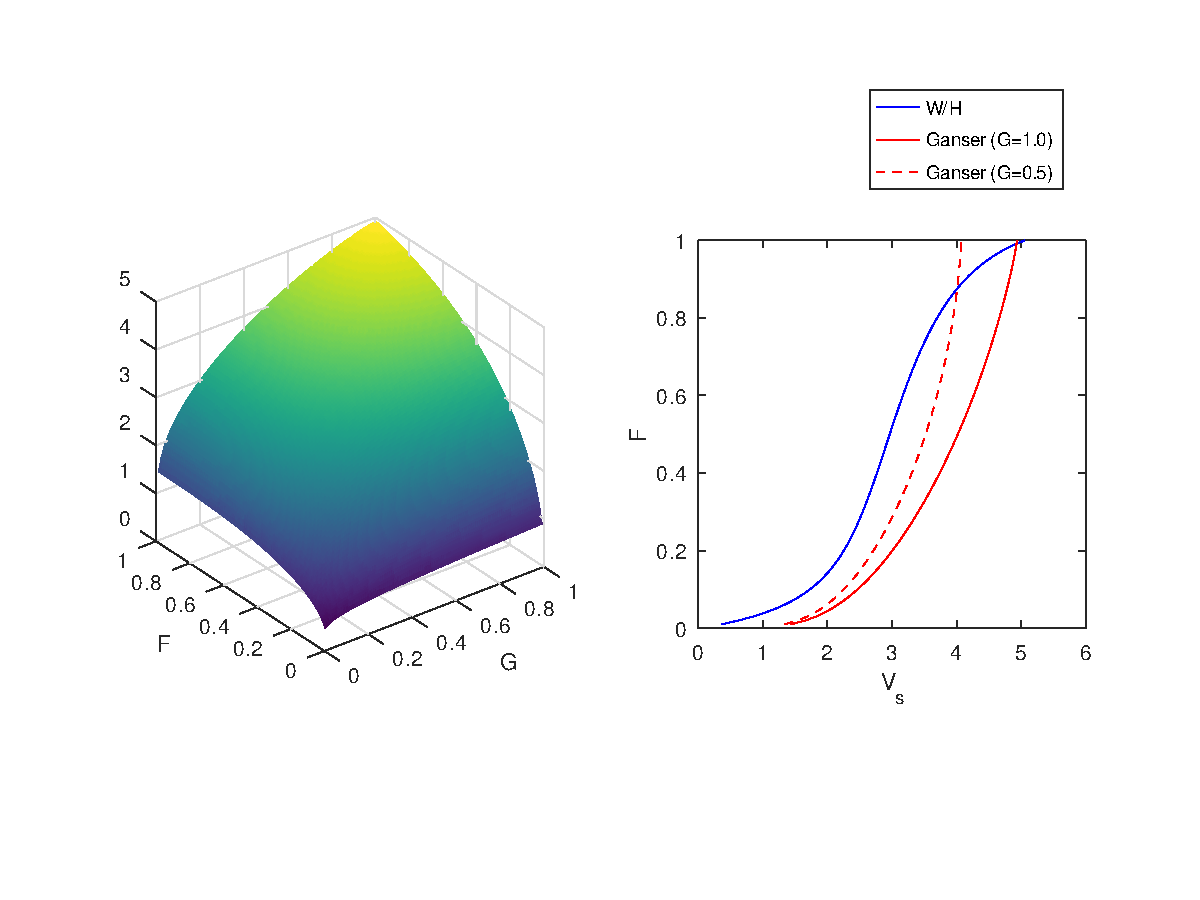
\includegraphics[angle=0,scale=0.6]{Figures/Scripts/FallMech/FigFVd500.pdf}
\parbox{15cm}{\caption{\label{FigFVd500}
Wilson/Huang and Ganser models of fall velocity for $d=1\,\mathrm{mm}$
with atmospheric conditions at $5\,\mathrm{km}$ height.}}
\end{figure}
\begin{figure}[htbp]
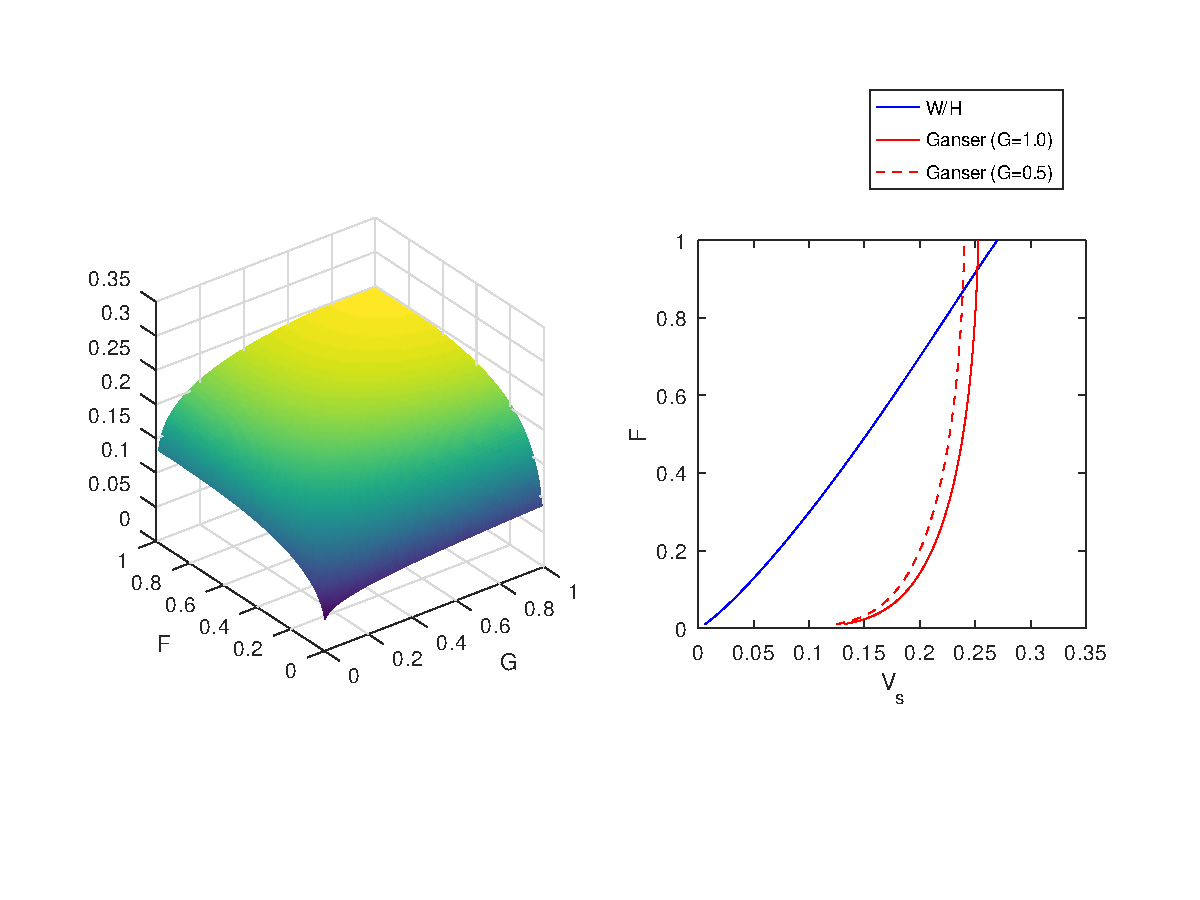
\includegraphics[angle=0,scale=0.6]{Figures/Scripts/FallMech/FigFVd064.pdf}
\parbox{15cm}{\caption{\label{FigFVd500}
Wilson/Huang and Ganser models of fall velocity for $d=64\,\mathrm{\mu m}$
with atmospheric conditions at $5\,\mathrm{km}$ height.}}
\end{figure}



%I thought a bit about our discussion of the sensitivity of Ash3d fall velocities
%to the shape factor $F$ and why it is so much more sensitive than you would expect.
%Roger and Alexa, I thought you might be interested in this discussion as well
%since it opens up some of the subtleties of how we specify a particle size in
%Ash3d.  There are a few fall models we have available in Ash3d
%(Stokes, Wilson/Huang, Ganser) which use different measures of diameter.
%The 'd' that we enter in the input file is the 'd' used in the fall model.
%Stokes is simply the diameter of the sphere (d0), the Ganser model is based the
%ratios ellipses to spheres of equivalent volume (dv turns out to be the geometric
%average of the 3 axies of the ellipsoid), and W/H uses the arithmetic average (da).
%This means that using the W/H model for a given 'd' with a low F (highly eccentric),
%the corresponding volume is significantly lower than the equant particle volume.
%So perturbing F to a lower value means you are both perturbing the shape (leading
%a greater drag) as well as perturbing the mass to a lower value.  These coupled
%effects both lead to slower fall velocities, resulting in a high sensitivity to F.
%The Ganser model should not be as susceptible to this since it separates mass and
%shape.  Shape in the Ganser model, by the way, probably should be specified
%through dv, but the actual implementation currently is a bit convoluted since it
%assumes 'd' = A and that B=C (no pancakes, only cigars).
%
%To see how big of a deal this is, I set up a matlab script (attached) that
%calculates F and Vf for a specified 'd' using the W/H model, but considering
%the input value of 'd' to be either da (as needed by W/H), or as dv which is
%converted to a da before calculating the W/H Vf.  So in the example attached,
%I assume an input diameter of 50 um, then consider a range of B and C axis
%lengths from some small value up to 50 um and calculate the length of A such
%that da = 50 um or that dv = 50 um.  From these A, B, C values you can calculate
%F\_a (shape assuming a constant da) and F\_v (shape assuming a constant Vol).
%These F values lead to their own ranges in Vf.  Bottom line from decoupling
%shape and volume (or mass) is that shape can still be a big factor (Vf\_v
%normalized to equivalent sphere is 0.6 for an F of 0.45).  Assuming a
%constant da, a normalized Vf\_a is closer to 0.5 for an F of 0.45.  The
%pattern changes negligibly for sea level and 20km and minimally for different
%particle sizes.
%
%I've attached the figures for F and Vf for these assumptions along with the
%script (and supporting scripts).
%
%So this begs the question: Should we change the interpretation of 'd' in the
%input file?  Currently, it is interpreted differently depending on the fall
%model.  We could specify a fixed interpretation then convert to whatever d is
%needed for the specified fall model.  Options for this would be:
%
%1) da
%This would change nothing for W/H or Stokes models, but would be problematic for Ganser
%
%2) dv
%This seems to me to be a more natural measure.  It would require a trivial
%conversion to da for W/H but would also mean that all past model input files
%would produce different results.
%
%3) A
%This would mean that 'd' reflect the largest length scale of the particle, but
%may not be that meaningful for needle-like particles
%
%4) B
%This is also a nice measure since it reflects what if determined from a sieve
%analysis.
%
%5) something else in line with a laser diffraction measurement.
%
%If we were starting from scratch, I would suggest option 2.  Given that we
%already have so many results assuming 'd' = da, I suggest that we leave the
%interpretation of 'd' to be model-specific and that I fix the Ganser model so
%that 'd' = dv instead of A and that it accepts two shape parameters F1=B/A
%and F2=C/A.
%%%%%
%Initially, we calculated the settling velocity by initializing the fall velocity
%as 1 m/s, calculating Re with this velocity, then Cd from this Re, and iteratively
%calculating a new velocity (and subsequent new Re and Cd) until the difference
%between the old and new velocities was less than some fraction.  We used 0.1\%
%and found it converged fairly quickly.  As you point out, the equations for the
%W/H model can be combined into a quadratic so we now use that.  One root is
%always negative so choose the positive root, which agreed with the iterative solution.
%
%The Ganser and Pfeiffer models cannot be simplified as nicely as the W/H model
%so we must use the iterative approach.  For the Ganser model, we calculate Cd
%from Eq 18 from his paper.  For this we need K1 and K2 which we get from
%Table 7 using the isometric equations.  The non-isometric equation only effects
%the Stokes term and requires knowing the ratio of diameters of spheres of
%equivalent projected area to one of equivalent volume.  I don't know how one
%would know the projected area of a tumbling particle so we just go with the
%isometric case and accept the errors for tumbling cigars and pancakes.  The
%D is needed for calculating the fall velocity of a particle in a tube.  The
%correction term to account for the effect of the tube walls has D in the
%denominator.  That term vanished as the tube diameter gets larger so we assume
%it away.
%
%K1 and K2 require knowing the sphericity (phi) which is the ratio of the
%surface area of a sphere of equivalent volume to the actual surface area
%of the particle.  Here's where we make some assumptions.  We interpret the
%shape term in the input file to be the shape factor F from the W/H model.
%This is simply the ratio of the average of the minor axes to the major axis
%of the ellipse (we assume all particles to be ellipses).  I wanted that
%shape factor have the same meaning as W/H so that the user can easily toggle
%between fall models.  The W/H model will produce the same answer for different
%ellipses as long as 0.5*(b+c) is the same.  The Ganser model can distinguish
%between pancakes and cigars, but we would need information about how b and c
%differ. Currently, we just use the one shape factor F and assume b=c
%(i.e. cigars only).  We can then use F to calculate the surface area,
%volume of the ellipsoid and surface area of a sphere of equivalent volume
%(and therefore phi) as a function of the major axis.  So the particle size
%we read from the input file is the length of the long axis of the ellipse.
%This is also the length term that we use in the calculation of Re.
%Wilson and Huang have a discussion about the best length measure to use
%for Re at the end of section 3, but we simply use the long axis.
%
%Buoyancy effects are minimal since the density contrast between ash and air is so large.
